\chapter{Suggested Algorithms}
\label{chapter_solutions}

% **************************** Define Graphics Path **************************
\ifpdf
    \graphicspath{{Chapter4/Figs/Raster/}{Chapter4/Figs/PDF/}{Chapter4/Figs/}}
\else
    \graphicspath{{Chapter4/Figs/Vector/}{Chapter4/Figs/}}
\fi

This chapter presents the suggested learning algorithms for predictive models in detail. First section \ref{sec_formalProblemDef} defines the problem of predicting events in a stream formally. Subsequently sections \ref{sec_predictiveEpisodeMining} and \ref{sec_FeatureBasedStreamWindowClassification} explain the two approaches suggested by this thesis, which are called predictive episode rule mining and feature based stream window classification. Finally section TODO explains how the models created by these methods can be evolved as the stream progresses.

\section{Formal Problem Definition}
\label{sec_formalProblemDef}
The problem to be tackled in this thesis is the prediction of future events in data streams using episode patterns. The approaches shall have the following properties:

\begin{itemize}
	\item \textbf{Local and fast prediction:} We do not focus on long term trends or on predictions of special values at fixed times (for example daily closing values of stocks), but instead aim to give predictions about the near future given the current state of the stream.
	\item \textbf{Usage of a Stream of categorical Values} Most forecasting methods focus on regression, meaning the predictions of numerical values. In contrast to this we work on streams of categorical events and we aim to predict the occurrences of events of certain types.
\end{itemize}

In this context we define:

\begin{mydef}
\textbf{Categorical Event Stream} A categorical event stream is defined as a (possibly infinite or constantly updating) sequence: $S = [ (T_1,t_1),(T_2,t_2),... ] $ where $T_i \in \Sigma$ is the event type of the i-th event and $t_i \in \mathbb{N}^+$ is the timestamp of the i-th event. The sequence is ordered according to the timestamps, which means that $\forall i,j \in {1,...,n} \; i<j \implies t_i \leq t_j$.
\end{mydef}

Note that this definition is essentially the same as definiton \ref{def_eventSequence}, which defines event sequences. The only difference is that in a categorical event stream we allow new events to constantly come in, which makes the sequence possibly infinite. Given a categorical event stream it is the goal of this thesis to develop algorithms that will build predictive models:

\begin{mydef}
\label{def_predictiveModel}
\textbf{Predictive Model} A predictive model for $M(T)$, $T \in Sigma$ is a model that if given a window $W$ (see definition \ref{def_timeWindow}) of a categorical event stream will output a binary value in the following:
\begin{itemize}
	\item $1$ if the model expects an event of type $T$ to occur shortly after $W$.
	\item 0 otherwise.
\end{itemize} 
\end{mydef}

Definition \ref{def_predictiveModel} purposefully remains vague about what \textit{"shortly after"} means mathematically, since this may depend on the underlying stream, or the users intent. Usually this will mean something like \textit{"x time units in the future"} or \textit{"at most x time units in the future"}

\section{PERMS - Predictive Episode Rule Mining in Streams}
\label{sec_predictiveEpisodeMining}
The first suggested algorithm is called the PERMS algorithm, short for \textbf{P}redictive \textbf{E}pisode \textbf{R}ule \textbf{M}ining in \textbf{S}treams.

\subsection{Basic Ideas and Definitions}
In order to fully explain the algorithm we first need to define what we mean by predictive episode rules.

\begin{mydef}
\label{def_predictiveEpisode}
\textbf{Predictive Episode Rule} An episode $\alpha$ is called a predictive episode rule for event $A \in \Sigma$ if $\alpha$ has the form $\beta \rightarrow A$ where $\beta$ is an episode. In this context we also refer to $\beta$ as the prefix or predictor and to $A$ as the suffix or target event of $\alpha$. 
\end{mydef}

%<<<<<<< HEAD old version? - pretty sure old version
%In the context of a predictive episode rule $\alpha = \beta \rightarrow A$ we also refer to $\beta$ as the prefix and to $A$ as the suffix or target event of $\alpha$.
%The basic idea of the prediction algorithm using predictive episode rules is rather simple. If given a set $P$ of predictive episode rules, we monitor the stream and whenever we detect the prefix of an episode in $P$ we predict an occurrence of $A$. The idea is similar to the mining of sequential rules or rule-based classification (TODO: cite). In principle $A$ does not need to be a single event label but could also be a more complex structure, like an episode. In this thesis we restrict ourselves to single events as suffixes for predictive episode rules.
%Of course there is an infinite amount of predictive episode rules for an event type, finding those predictive episode rules that are actually useful for predicting the occurrence of an event is the main task when building (training) the model. The use case here is very similar to the related work that deals with the constraint based mining of episode rules (TODO: cite), where episode rules are mined in order to discover dependencies between earthquakes. There are two main important differences that make the approach used by the authors (TODO: name them) impractical.
%=======
The basic idea of the prediction algorithm using predictive episode rules is rather simple. If given a set $P$ of predictive episode rules, we monitor the stream and whenever we detect the prefix of an episode in $P$ we predict an occurrence of $A$. The idea is similar to the mining of sequential rules or rule-based classification \cite{ma1998integrating}.
Of course there is an infinite amount of predictive episode rules for an event type, finding those predictive episode rules that are actually useful for predicting the occurrence of an event is the main task when building (training) the model. The use case here is very similar to the related work that deals with the constraint based mining of episode rules \cite{meger2004constraint}, where episode rules are mined in order to discover dependencies between earthquakes. There are two main important differences that make the approach used by the authors impractical:

\begin{itemize}
 \item We are interested in episode rules of one specific type (those predicting the desired event $A$), thus it is not necessary to mine all frequent episode rules in the stream.
 \item We are dealing with data in a streaming environment, meaning we can neither analyze the whole data, nor make multiple passes over the entire stream.
\end{itemize}

In order to describe how the set $P$ is built by the suggested learning algorithm,we first need to define frequency, support and confidence for predictive episode rules, which are similar to classic association rules \cite{agrawal1994fast}. Before this can be done however we need to determine which frequency definition we will use in this algorithm. 

\subsection{Choice of Frequency Measure}

Recall that there are three main frequency measures that were proposed in the literature:

\begin{itemize}
	\item The Window-based Frequency (see defintion \ref{def_windowBasedFrequency})
	\item The frequency based on minimal occurrences (see definition \ref{def_minimalOccuranceFrequency})
	\item The frequency based on non-overlapping occurrences (see definition \ref{def_nonOverlappingFrequency})
\end{itemize}

Their properties were already discussed in subsection \ref{subsec_otherFrequency}. While the frequency measure using the non-overlapping occurrences is the latest measure and offers the best theoretical runtime, when recognizing episodes in a sequence it has a few drawbacks that are detrimental to its use in the given scenario. The first one is that it does not limit the duration of the episode occurrences. However limiting the duration of episode rules, or in other words giving episode occurrences expiry times is necessary when predicting event occurrences in streams. Consider for example the simple predictive episode rule $\alpha = B \rightarrow A$ and the following example sequence: 

\begin{equation}
S = [ (B,1),(C,2),(A,3),(B,4),...,(A,2000) ] 
\end{equation}

The non-overlapping frequency definition recognizes both $(B,1) \rightarrow (A,3)$ and $(B,4) \rightarrow (A,2000)$ as equally valid occurrences of $\alpha$ in $S$. However it is to be expected that when looking for episode rules for predictive purposes in a stream the events should happen close to each other (time-wise). This means that in this case $(B,1) \rightarrow (A,3)$ is likely a correct occurrence and prediction, whereas the occurrence $(B,4) \rightarrow (A,2000)$ is simply owed to the fact that at some point of time event $A$ will occur again in the stream and $(B,4)$ happened to occur a long time before that, without there necessarily being a correlation or causality.
Additionally the non-overlapping frequency assumes that there is one long sequence, from which the episodes are to be mined. The window-based frequency however works on a set of individual windows of a sequence or stream. In the previous work this had not been an advantage or disadvantage, since it did not focus on the streaming scenario, which meant that it was possible to analyze the entire sequence. This lead to the use of sliding windows over the sequence when using the window-based frequency. In the streaming scenario it is impossible to use all of the data, instead a certain selection is necessary. This can be done easily when using the window-based frequency by simply storing the windows that are of interest. Selecting data for the non-overlapping frequency definition is more difficult. Thus we will use the window-based frequency in this approach

\subsection{Basic Definitions}
Since we decided on a frequency measure it is now possible to define frequency, support and confidence of predictive episode rules.

\begin{mydef}
\label{def_frequency}
\textbf{Frequency} If given a set of time windows $WIN$ (see definition \ref{def_timeWindow}) of a sequence or stream the frequency of a predictive episode $\alpha$ is defined as the number of windows in which $\alpha$ occurs: $freq(\alpha) = |\{W\,|W \in WIN\; \land \alpha\; occurs \; in \; W\}|$
\end{mydef}

\begin{mydef}
\label{def_support}
\textbf{Support} If given a set of time windows $WIN$ of a sequence the support of a predictive episode $\alpha$ is defined as $s(\alpha) = \frac{freq(\alpha)}{|WIN|}$
\end{mydef}

\begin{mydef}
\label{def_confidence}
\textbf{Confidence} The confidence of a predictive episode $\alpha = \beta \rightarrow A$ is defined as $c(\alpha) = \frac{s(\alpha)}{s(\beta)}$ \cite{meger2004constraint}
\end{mydef}

The intention is clear and similar to the mining of classic association rules \cite{agrawal1994fast}: If a rule has a high confidence, it means that the prefix of the rule rarely occurs without its suffix $A$, meaning there is a high chance that this is a true predictor for the event $A$. Thus the goal of PERMS is to find a set of predictive episode rules $P$ that have a very high confidence and are above a certain support limit.

\subsection{Choice of training data}
Recall that in streaming applications it is impossible to analyze the whole stream as one sequence using multiple passes. Thus, when presented with a stream any prediction or forecasting algorithm first needs to take some time to study the stream and extract training data to build the model. So if given a categorical event stream, how do we determine the training data? As it was described in section \ref{sec_episodeMiningBackground} the data basis for episode mining is one very long sequence. Thus the first simple approach would be to simply record the stream as a sequence until we have reached a number of desired elements or run out of memory. The recorded sequence would then be the training sequence from which the predictive episode rules can be mined. This approach is visualized in figure \ref{fig_trainingDataNaive}.

\begin{figure}[h]
	\centering
  	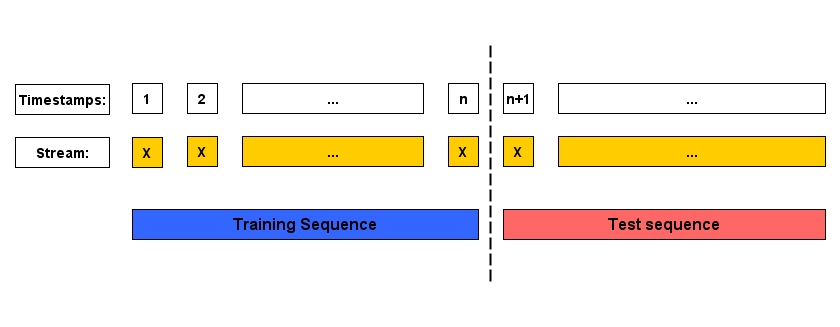
\includegraphics[width=\textwidth]{trainingDataNaive}
	\caption{Visualization of a simple split of the stream into a training segment at the beginning, followed by a (potentially endless) test phase}
	\label{fig_trainingDataNaive}
\end{figure}

The disadvantage of this naive approach is that there is no guarantee about the number of occurrences of the event we aim to predict. Say we want to predict $A$ and $A$ is rather sparse in the beginning of the stream, then we will have a very small data basis to extract predictive episode rules for $A$ and thus will likely not succeed. 
A better approach is to keep a window of the stream a certain duration $d$ in memory and scan the stream for occurrences of the target event $A$. Whenever an event of type $A$ enters the window we store the current window in a list until we have a sufficient number of windows. This approach is visualized in figure \ref{fig_trainingDataWindowsOfA}. It guarantees that we have a sufficient number of windows that are immediately followed by the target event. The mining process then is to simply find frequent episodes in the mined windows. Each of these then automatically corresponds to the prefix of a potential predictive episode rule with the suffix being the target event ($A$ in the figures). The window duration $d$ is at the same time the maximum duration for episode occurrences.

\begin{figure}[h]
	\centering
  	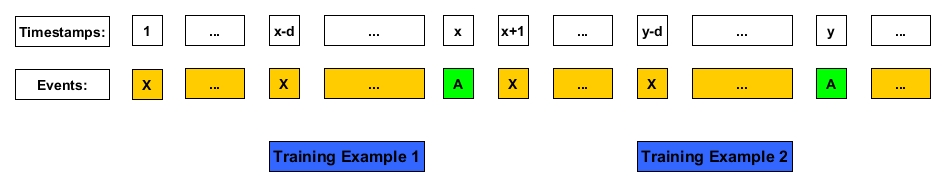
\includegraphics[width=\textwidth]{trainingDataWindowsOfA}
	\caption{Visualization of using fixed windows that precede the target event as training examples. Predictive episodes can be mined from the windows that are extracted from the stream as shown above.}
	\label{fig_trainingDataWindowsOfA}
\end{figure}

The obvious and very big disadvantage is that there are no negative examples in the training sample taken from the stream. Each window is immediately followed by the target event $A$, thus every episode mined from the windows can have $A$ appended as a suffix and thus every predictive episode rule will have a confidence of $1.0$. This means that selection via confidence is meaningless, since we have seen no negative examples, meaning windows that are not followed by $A$. However negative examples can be extracted from the stream in a similar manner. This results in $m$ positive examples, also referred to as positive windows, which are followed by $A$ and $m$ negative examples, also called negative windows, which are not followed by $A$. This is the basic idea behind the training data selection in PERMS. It is visualized in figure \ref{fig_trainingDataPositiveAndNegativeWindows}. 

\begin{figure}[h]
	\centering
  	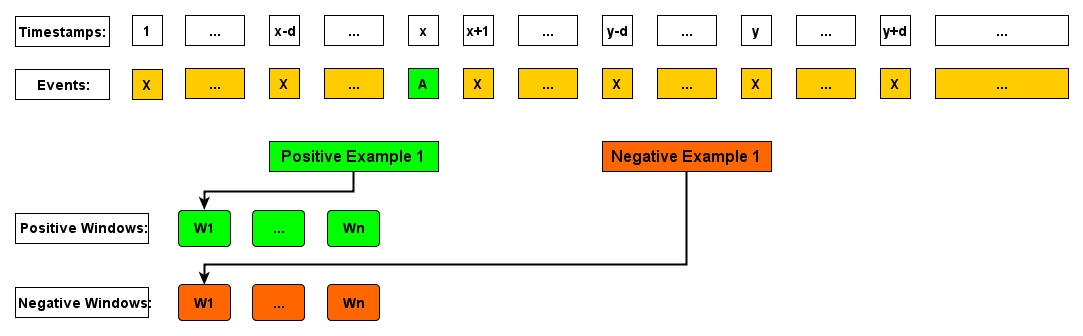
\includegraphics[width=\textwidth]{trainingDataPositiveAndNegativeWindows}
	\caption{Extracting positive and negative example windows from the stream.}
	\label{fig_trainingDataPositiveAndNegativeWindows}
\end{figure}

In order to make sure, that none of the patterns in the negative windows are followed by event $A$, even if the occur right before the end of the window, we demand that after the negative window $A$ does not occur in the next $d$ time units. This means that we need to keep a window of the stream, that has $2\cdot d$ duration.\\
There are still some issues with this approach that can be detrimental to the predictive performance of the model. One issue is that we extract an equal amount of positive and negative windows from the stream with no respect to the original distribution. If $A$ occurs very rarely, having an equal amount of positive and negative examples in the training data does not reflect the original event distribution in the stream. If that is the case, this can be fixed by including a number of negative examples that is proportionate to the original distribution (which is either known or learned while extracting the training data). However it is unclear if that would actually have a significantly positive effect on the performance of the resulting model. \\
This approach is actually similar to the approach of Laxman et. al. as described in their paper about generative models for prediction in streams \cite{laxman2008stream}. They do however only consider serial episodes and focus on learning hidden markov models in order to predict events, as opposed to finding episode rules.

\subsection{PERMS Parameters and Pseudocode}
\label{subsec_perms}

The PERMS algorithm uses the following user-defined parameters:

\begin{itemize}
	\item \textbf{$d$} - the duration of the sliding window. This also implies that all windows which the predictive episode rules will be mined from will exactly have duration $d$.
	\item \textbf{$m$} - the number of positive windows to mine the predictive episode rules from. This means that we will mine $m$ positive and $m$ negative training examples from the stream.
	\item \textbf{$s$} - the minimum support that predictive episode rules must have to be considered for the model (rules with support $s$ or higher are frequent).
	\item \textbf{$n$} - the desired size of the final set of predictive episodes, also referred to as the ensemble size.
\end{itemize}

The pseudocode for PERMS is given in algorithm \ref{alg_PERMS}. Recall that for formally accessing episodes we use the notation introduced in subsection \ref{subsec_basicEpisodeDefinitions}.

\begin{algorithm}[H]
  \caption{PERMS
    \label{alg_PERMS}}
  \begin{algorithmic}[1]
    \Statex
    \Require Let $S=[(T_s,t_1),...]$ be a stream of events and let $d$,$m$,$s$,$n$ be the parameters as defined in the beginning of subsection \ref{subsec_perms}.
    \Function{PERMS}{}
      \Let{$(PE,NE)$}{$WindowMining(S,d,m,A)$} 
      \Let{$P$}{$BuildPredictiveEpisodeModel(PE,NE,s,n)$}
      \State apply Set of predictive Episodes $P$ to the rest of the Stream $S$
    \EndFunction
  \end{algorithmic}
\end{algorithm}

As seen in the algorithm above the basic idea of the PERMS algorithm can be divided into 2 parts: training example mining (window mining) and predictive episode model building. To mine the training examples we start at the beginning of the stream and keep a sliding window of a user defined duration $d$ in memory (see definition \ref{def_timeWindow}. Whenever an event of type $A$ enters the window we store the current window in a list until we have a sufficient number of windows ($m$). Additionally we also store $m$ windows that do not contain $A$ and were also not followed by $A$ in the near future. The pseudocode for this is given in algorithm \ref{alg_traningExampleMining}.

\begin{algorithm}[H]
  \caption{Training Example Mining
    \label{alg_traningExampleMining}}
  \begin{algorithmic}[1]
    \Statex
    \Require Let $S=[(T_s,t_1),...]$ be a stream of events, $d$ be the window duration, $m$ the required number of windows and $A$ the event type to predict.
    \Function{WindowMining}{}
      \Let{$PE$}{$\emptyset$} 
      \Let{$NE$}{$\emptyset$}
      \Let{$i$}{$1$}
      \Let{$t_{last}$}{$t_1$}
      \While{$|PE| \neq m \; \lor |NE| \neq m $}
      	\Let{$(T_i,t_i)$}{$S[i]$}
      	\If{$T_i = A$}
      		\Let{$t_{last}$}{$t_i$}
      		\If{$|PE| \neq m$}
          		\Let{$PE$}{$PE \cup W(S,i-d-1,i-1)$}
          	\EndIf
		\ElsIf{$|NE| \neq m \; \land t_i - t_{last} \geq d\cdot 2$}
			\Let{$NE$}{$NE \cup W(S,i-d \cdot 2,i-d)$}
			\Let{$t_{last}$}{$t_i$}
       	\EndIf
       	\Let{$i$}{$i+1$}
      \EndWhile
      \State \Return{$(PE,NE)$}
    \EndFunction
  \end{algorithmic}
\end{algorithm}

Once we have enough training examples, we can start to mine serial and parallel episodes from the windows preceding $A$ that have support $s$ or higher. For that purpose we employ the general mining algorithm for frequent episodes (see algorithm \ref{alg_generalEpisodeMining} in subsection \ref{subsec_episodeDiscovery} ). In addition to a frequency measure, this algorithm requires counting algorithms for episode frequency. The existing algorithms for counting episode frequency are made for the use case of one long sequence being mined for frequent patterns instead of single windows. Thus they are rather complex, since they avoid recounting the frequency of a candidate episode for each window and instead update counts when sliding the window forward \cite{mannila1997discovery}. Since the windows in our use case are not necessarily back to back, we can simplify the episode detection algorithms to work on one window only and simply apply them to each window for each episode. The simplified detection algorithms for serial and parallel episodes are shown in algorithms \ref{alg_SerialEpisodeDetection} and \ref{alg_ParallelEpisodeDetection}. Afterwards we rank the discovered rules by confidence, keep the $n$ episodes with the highest confidence and return them as the set of predictive episodes $P$. The pseudocode for this is given in algorithm \ref{alg_BuildPredictiveEpisodeModel}.

\begin{algorithm}[H]
  \caption{Predictive Episode Model Building
    \label{alg_BuildPredictiveEpisodeModel}}
  \begin{algorithmic}[1]
    \Statex
    \Require Let $PE$ be the positive examples (Windows preceding $A$), let $NE$ be the negative examples (Windows not followed by $A$). Furthermore let $s$ be the minimum support and $n$ the number of predictive episodes to keep.
    \Function{BuildPredictiveEpisodeModel}{}
      \Let{$P$}{$MineFrequentParallelEpisodes(PE,s)$} 
      \Let{$S$}{$MineFrequentSerialEpisodes(PE,S)$} 
      \Let{$E$}{$P \cup S$}
      \For{each $\alpha \in E$}
      	\Let{$\alpha .c = calcConfidence(\alpha,PE,NE)$}
      \EndFor
      \State Sort the $\alpha \in E$ by  $\alpha .c$
      \State \Return{the top $n$ episodes $\alpha \in E$}
    \EndFunction
  \end{algorithmic}
\end{algorithm}

\begin{algorithm}[H]
  \caption{Serial Episode Detection in one Window
    \label{alg_SerialEpisodeDetection}}
  \begin{algorithmic}[1]
    \Statex
    \Require Let $W=[(T_s,t_1),...,(T_e,t_n)]$ be a Window of the Stream and let $\alpha$ be a serial episode.
    \Function{SerialEpisodeDetection}{}
      \Let{$i$}{$1$}
      \Let{$pos$}{$1$}
      \Let{$t_{prev}$}{$-1$}
      \While{$i \leq |W| \land pos \neq |\alpha |$}
      	\Let{$(T_i,t_i)$}{$W[i]$}
      	\If{$T_i = \alpha [pos] \; \land t_i \neq t_{prev}$}
      		\Let{$t_{prev}$}{$t_i$}
      		\Let{$pos$}{$pos+1$}
        \EndIf
       	\Let{$i$}{$i+1$}
      \EndWhile
      \State \Return{$true$ if $pos =|\alpha |$, $false$ otherwise}
    \EndFunction
  \end{algorithmic}
\end{algorithm}

\begin{algorithm}[H]
  \caption{Parallel Episode Detection in one Window
    \label{alg_ParallelEpisodeDetection}}
  \begin{algorithmic}[1]
    \Statex
    \Require Let $W=[(T_s,t_1),...,(T_e,t_n)]$ be a Window of the Stream and let $\alpha$ be a parallel episode.
    \Function{ParallelEpisodeDetection}{}
      	\Let{$i$}{$1$}
      	\Let{$removed$}{$0$}
      	\Let{$Remaining$}{new empty Map}
		\For{each $A \in \alpha$}
      		\Let{$Remaining[A]$}{$count(\alpha,A)$}
      	\EndFor      
      \While{$i \leq |W| \; \land removed \neq |\alpha |$}
      	\Let{$(T_i,t_i)$}{$W[i]$}
      	\If{$T_i \in \alpha \;\land Remaining[T_i] \neq 0$}
      		\Let{$Remaining[T_i]$}{$Remaining[T_i] - 1$}
      		\Let{$removed$}{$removed + 1$}
        \EndIf
       	\Let{$i$}{$i+1$}
      \EndWhile
      \State \Return{$true$ if $removed =|\alpha |$, $false$ otherwise}
    \EndFunction
  \end{algorithmic}
\end{algorithm}

After selecting the best $n$ predictive episodes the model can be applied to the rest of the stream.
The application of the predictive model to the stream is very simple: If an episode $\alpha \in P$, with $P$ being the set of best predictive episodes, occurs in the current sliding window output $1$ and otherwise output $0$ for the current sliding window.

%\begin{algorithm}[H]
%  \caption{Calculate Window based Frequency for parallel Episodes
%    \label{alg_windowBasedParallel}}
%  \begin{algorithmic}[1]
%    \Statex
%    \Require Let $C$ be the set of candidate parallel episodes, and let $S=[(T_1,t_s),...,(T_n,t_e)]$ be a sequence of events, let $win$ be the window size and finally let $minS$ be the minimum support.
%      \State \textit{// Initialization}
%      \For{each $\alpha \in C$}
%      	\For{each $A \in \alpha$}
%      		\Let{$A.count$}{$0$}
%      		\For{$i \in \{1,...,|\alpha |\}$}
%      			\Let{$contains(A,i)$}{$\emptyset$}
%      		\EndFor
%      	\EndFor
%      \EndFor
%      \For{each $\alpha \in C$}
%      	\For{each $A \in \alpha$}
%      		\Let{$a$}{number of events of type $A$ in $\alpha$}
%      		\Let{$contains(A,a)$}{$contains(A,a) \cup \{\alpha \}$}
%      	\EndFor
%      	\Let{$\alpha .eventCount$}{$0$}
%      	\Let{$\alpha .freq$}{$0$}
%      \EndFor
%      \State \textit{// Recognition}
%      \For{$start \gets t_s - win +1 \textrm{ to } t_e$}
%      	\State \textit{//Bring new events to the window}
%      	\For{each $(t,A) \in S $ where $t = start+win-1$}
%      		\Let{$A.count$}{$A.count +1$}
%      		\For{each $\alpha \in contains(A,A.count)$}
%      			\Let{$\alpha .eventCount$}{$\alpha .eventCount + A.count$}
%      			\If{$\alpha .eventCount = |\alpha | $}
%          			\Let{$\alpha .inwindow$}{$start$}
%       			\EndIf
%      		\EndFor
% 		\EndFor
% 		\State \textit{// Drop old events out of the window}
% 		\For{each $(t,A) \in S $ where $t = start-1$}
% 			\For{each $\alpha \in contains(A,A.count)$}
% 				\If{$\alpha .eventCount = |\alpha | $}
%          			\Let{$\alpha .freq$}{$\alpha .freq + \alpha .inwindow -start $}
%       			\EndIf
%       			\Let{$\alpha .eventCount$}{$\alpha .eventCount - A.count$}
% 			\EndFor
% 			\Let{$A.count$}{$A.count -1$}
% 		\EndFor
%      \EndFor
%      %\Let{$freq$}{$\emptyset$}
%      %\Let{$i$}{$1$}
%      %\While{$C_i \neq \emptyset$}
%      	%\State Count frequencies of each Episode $E \in C_i$
%       % \Let{$L_i$}{ $\{ E \mid E \in C_i \land C_i \; is\; frequent\}$}
%       % \Let{$freq$}{$freq \cup L_i$}
%       % \Let{$C_{i+1}$}{Generate Episode Candidates of length $i+1$ from $L_i$}
%        %\Let{$i$}{$i+1$}
%      %\EndWhile
%      \State \Return{$\{\alpha \mid \alpha \in C \land \frac{\alpha.freq}{t_e - t_s + win -1} \geq minS\}$}
%  \end{algorithmic}
%\end{algorithm}

\subsection{Theoretical Complexity}
\label{subsec_permsComplexity}
It is best to analyze the runtime and space requirements of PERMS for each step individually. The first step, meaning the mining of training examples (see algorithm \ref{alg_traningExampleMining} ) requires a sliding window over the stream. Runtime obviously depends on how long we need to scan the stream until we have a sufficient number of training windows. Since this is dependent on the use-case we refer to the length of the stream that needs to be processed until we have extracted all training examples as $S_T$. Additionally we need to store all training examples. If we assume that the size of a training window is $\Theta(|W|)$ we require $\Theta(S_T + m\cdot |W|)$ time and $\Theta(m\cdot |W|)$ space. The exact size of a training window is obviously dependent on the stream's properties, such as velocity (with a high velocity, there will be more events happening in the duration of $d$ than with a low velocity). If we assume that per timestamp there can be at maximum one event of each type we can use the following upper bound for the size of a window: $|W| = O(d\cdot |\Sigma|)$ as the worst case. \\
The majority of the training time is expected to be spent in the pattern mining phase. As with all pattern mining approaches, mining frequent episodes suffers from the problem of pattern explosion, meaning if the desired minimum support is too low, the algorithm will require exponential time and space. It is therefore usual to denote the the number of candidate episodes of length $i$ for which frequencies need to be counted as $|C_i|$. We say that $C_i$ contains all parallel and all serial episodes of size $i$. Furthermore we say that $|C| = \sum_{i=1}^N |C_i|$ is the total number of candidates ($N$ being the maximum episode length that needs to be considered). As it can be seen in algorithm \ref{alg_generalEpisodeMining}, we need to count the frequency of each candidate episode once. In order to count the frequency, we need to determine whether a candidate episode occurs in a window, which in the worst case means that we need to loop through the entire window and the entire episode (see algorithms \ref{alg_ParallelEpisodeDetection} and \ref{alg_SerialEpisodeDetection}). Thus we arrive at $\Theta(|C_i| \cdot m \cdot(|W| + i))$ runtime to count frequencies for $C_i$. This gives us an upper bound for the total runtime, which is: $O(|C| \cdot m \cdot(|W| + N))$. Similarly we get the upper bound for of $O(|C|\cdot N + m \cdot |W|)$ for required memory in total. If we make the slightly simplifying assumption that all episodes require constant space, we can simplify the runtime and memory requirements to $\Theta(|C| \cdot m \cdot |W| )$ for runtime and $\Theta(|C| + m \cdot |W|)$ for memory. Of course the required space for episodes rises with their length, however the assumption is still practical in a lot of cases, because:

\begin{itemize}
	\item Maximum Episode length typically remains very small.
	\item Efficient storage of episodes in Trie-like data structures can greatly reduce necessary space per episode in practice. For the efficient data structure see the section about technical realization TODO.
\end{itemize}

After having trained the model, predicting events in the current sliding window over the stream can be done naively in $O(n \cdot (|W|+N))$ time, since in each episode needs to be recognized and $O(n \cdot N + |W|)$ memory. The runtime can be optimized to $O(n \cdot N)$ (TODO: recheck this) by using continous automata for episode recognition as suggested by Mannila et. al. \cite{mannila1997discovery}. In practice this is pretty fast and also has the advantage that the recognition of the $n$ different episodes in the current sliding window can be parallelized if necessary.

\section{FBSWC - Feature Based Stream Window Classification}
\label{sec_FeatureBasedStreamWindowClassification}

The basic idea of the second approach called FBSWC, short for \textbf{F}eature \textbf{B}ased \textbf{S}tream \textbf{W}indow \textbf{C}lassification is similar to the one of PERMS. In fact the process of gathering training data as visualized in figure \ref{trainingDataPositiveAndNegativeWindows} is exactly the same. \\
In order to understand the approach of FBSWC, it is best to take a step back and see what we actually want to achieve. What we want to build is a predictive model that if given the current state of the stream can predict whether a target event $A$ will occur in the near future, or not. If we define the current state of the stream as a window $W$ containing the events of of up to $d$ time units into the past, we can easily formulate this problem as a binary classification problem of such time windows. The two classes are the two cases that we are interested in, which are:

\begin{itemize}
	\item $W$ is followed by $A$
	\item $W$ is not followed by $A$
\end{itemize}

\subsection{FBSWC Parameters and Pseudocode}

If we are able to map a window $W$ into a fitting feature space, we can train a feature based classifier on our training examples, whose mining is specified in algorithm \ref{alg_traningExampleMining}. The basic idea of FBSWC is to mine frequent episodes from both the positive as well as the negative examples, and then map each window to a feature space. The mapping works in the following: If $E$ is the set of frequent episodes, each episode will be mapped to a boolean feature, that is $true$ for an example $W$ if $\alpha$ occurs in $W$ and $false$ otherwise. It is clear, that unless the support parameter for the episode mining algorithm is very high, the resulting feature space will be too large for most feature based classifiers. Thus feature reduction approaches need to be employed before training the classifier. The algorithm for FBSWC is given in algorithm \ref{alg_FBSWC}.

\begin{algorithm}[H]
  \caption{FBSWC
    \label{alg_FBSWC}}
  \begin{algorithmic}[1]
    \Statex
    \Require Let $S=[(T_s,t_1),...]$ be a stream of events and let $d$,$m$,$s$ be the parameters as defined in the beginning of subsection \ref{subsec_perms}.
    \Function{FBSWC}{}
      \Let{$(PE,NE)$}{$WindowMining(S,d,m,A)$}
      \Let{$P_{PE}$}{$MineFrequentParallelEpisodes(PE,s)$} 
      \Let{$S_{PE}$}{$MineFrequentSerialEpisodes(PE,s)$} 
      \Let{$P_{NE}$}{$MineFrequentParallelEpisodes(NE,s)$} 
      \Let{$S_{NE}$}{$MineFrequentSerialEpisodes(NE,s)$} 
      \Let{$E$}{List of $(P_{PE} \cup S_{PE} \cup P_{NE} \cup S_{NE})$ in arbitrary, but fixed order}
      \Let{$T$}{List of $(PE \cup NE)$ in arbitrary but fixed order}
      \Let{$FS$}{new $T \times (|E|+1)$ Matrix} \Comment{Initializes the feature space}
      \For{$i \in \{1,...,|T|\}$}
      	\For{$j \in \{1,...,|E|\}$}
      		\Let{$FS[i,j]$}{$true$, if $E[j]$ occurs in $T[i]$, $false$ otherwise}
      	\EndFor
      	\Let{$FS[i,|E|+1]$}{$1$, if $E[j] \in PE$, $0$ otherwise} \Comment{Class Label}
      \EndFor
      \Let{$\widetilde{FS}$}{$FeatureSelection(FS)$}
      \Let{$M$}{$TrainFeatureBasedClassifier(\widetilde{FS})$}
      \State apply model $M$ to the rest of the Stream $S$
    \EndFunction
  \end{algorithmic}
\end{algorithm}

Note that in practice, the feature matrix $FS$ can be created while the frequent patterns are discovered, essentially eliminating the need for the loops from lines $10-13$. The FBSWC algorithm basically works with any feature selection approach, as well as with any feature based classifier. The choice is left open to the user.

\subsection{Theoretical Complexitiy}
The time and space needed to collect the training examples is identical to the one of PERMS, since FBSWC uses the same procedure.
Since FBSWC leaves the choices of feature selection and feature based classifier left to the user, we can not give clear runtime and memory bounds for the training step. If we assume that the feature selection algorithm takes $FS_T$ time and $FS_M$ memory and the feature based classifier takes $C_T$ time and $C_M$ memory, we can summarize the required runtime as $O(|C| \cdot m \cdot(|W| + N) + FS_T + C_T)$ and the memory as $O(|C|\cdot N + m \cdot |W| + |C|\cdot m + FS_M + C_M)$ for similar reasoning as in subsection \ref{subsec_permsComplexity}. The additional term $|C|\cdot m$ is necessary due to the feature matrix, which needs to be stored.


\section{Evolving the models with the stream}
\label{sec_EvolvingModels}

The 2 algorithms discussed so far are static learning algorithms, that once they passed the training phase do not change their behavior. This is often inappropriate in data streams, as models need to evolve as the stream progresses. There are a few possibilities for both algorithms to evolve with the stream.

\subsection{Evolving PERMS models}
Recall that a PERMS-model is essentially defined by a set of predictive episode rules. The prefixes of these rules were found to be frequent in the windows preceding the target event and the rules of the set were chosen to be part of the set on the basis of their confidence. The first step to an evolution of the model would be to introduce a second ensemble-size parameter $\tilde{n}$ that should be much larger than $n$. Instead of just keeping $P$ (the top $n$ predictors) in memory, PERMS now additionally keeps $\tilde(P)$, which is a set of $\tilde{n}$ other episode rules. These could be the next highest in confidence after $P$, but there could also be some benefit in randomizing parts of this set from all frequent predictors in order to maintain a diverse set. The idea is that as the stream progresses, new examples will be evaluated, which means that the confidence of the rules will change over time. This means that rules in $P$ that were initially good might lose their value over time and rules that were initially in $\tilde{P}$ might become better. By keeping track of these additional rules, one can immediately swap rules from $\tilde{P}$ to $P$, should their confidence become better than that of a rule in $P$. Additionally, if there is an overall decay in confidence this can signal that a complete re-training of the model might be necessary, since all of the rules in both $P$ and $\tilde{P}$ are no longer fitting. \\
This is of course something one wants to avoid since the training of the model can take a lot of time, depending on the support parameters. It would of course be ideal to keep track of all frequent predictors, while the stream is running. If that is possible re-training the model would become obsolete, since all frequent predictors with their confidences are known at any time. As mentioned in the previous work section about pattern mining in data streams \ref{subsec_PatternMining}, there is an approximation algorithm for maintaining all frequent itemsets in a data stream. The algorithm is known as the lossy-counting algorithm \ref{manku2002approximate}. In theory, the lossy-counting algorithm can be adapted to fit many kinds of patterns.  However, the problem with this algorithm is that the pruning of patterns is much weaker than in classical pattern mining, since many subfrequent patterns need to be kept in memory, because they might become frequent at some point of time. Since the problem of pattern explosion is generally worse for episodes, especially for serial episodes, as shown in section \ref{sec_PatternExplosion}, lossy counting might not be applicable to episode pattern mining in a lot of cases. As mentioned in section \ref{sec_episodes} mining algorithms to maintain the most frequent episodes in a time window over the stream have been developed recently. They could be applied to maintain the number of frequent episodes, however using these algorithms would mean that older training examples would have to be discarded as they leave the window.

\subsection{Evolving FBSWC models}
How FBSWC models can be evolved is essentially dependent on the feature based classifier that was chosen by the user. Many classifiers have already been adapted for the streaming environment. Among these are Decision Trees, Random Forests and Neural Networks (TODO: cite). Apart from evolving those classifiers, it is more difficult to evolve FBSWC, since classifiers usually can't change the feature space once they are trained. This means a switching of episode patterns like suggested for PERMS would require retraining the classifier on new features.